\documentclass[herrin-thesis.tex]{subfiles}
\begin{document}

\chapter{Data Collection and Processing}
\label{ch:data}

\section{Signal Readout}
\label{sec:data_signal_readout}
\begin{figure}
\centering
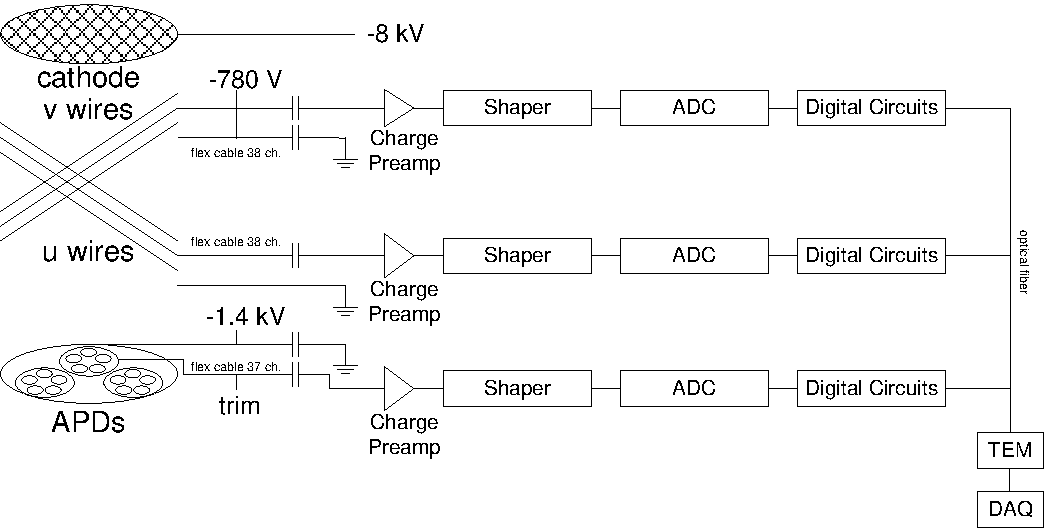
\includegraphics[width=\textwidth]{./figures/data_simplified_electronics.pdf}
\caption[The EXO-200 electronics]{A simplified schematic of the EXO-200 electronics. The ionization and scintillation signals are read out through long flex cables. The signals are shaped, digitized, and passed to the Trigger Event Module (TEM), which passes the data to the DAQ computers for recording when signals are detected.}
\label{fig:data_simplified_electronics}
\end{figure}

\begin{table}[tbp]
\centering
\caption[Electronic shaping times]{The shaping times for the signal readouts in EXO-200.}
\label{tab:data_shaping_times}
\begin{tabular}{l c @{\hskip 20pt} c c c @{\hskip 20pt} c c c}\toprule
							&&						\multicolumn{6}{c}{Stage Type}													\\\cmidrule{3-8}
	Channel Type				&&	\multicolumn{2}{c}{Integration (\si{\micro\s})}	&&	\multicolumn{3}{c}{Differentiation (\si{\micro\s})}				\\\midrule
	APDs					&&	3				&		3			&&	10				&	10				&	300			\\
	\multirow{2}{*}{\(u\) wires}		&&	\multirow{2}{*}{1.5}	&	\multirow{2}{*}{1.5}	&&	\multirow{2}{*}{40}	&	\multirow{2}{*}{40}	& 	measured 	\\
							&&					&					&&					&					& 	(nominally 60)	\\
	\(v\) wires					&&	3				&		3			&&	10				&	10				&	60			\\\bottomrule
\end{tabular}
\end{table}

\Cref{fig:data_simplified_electronics} shows a simplified schematic for the EXO-200 electronics. The APD signals and the ionization induction and collection signals are read out through long flex cables. The long cables separate the electronics from the TPC, removing the need for cryogenic and low-radioactivity components. After passing through a preamplifier, the signals are fed through shaping circuits and are then digitized at a rate of \SI{1}{\MHz}. The shaping circuits consist of two integrators followed by three differentiators. \Cref{tab:data_shaping_times} summarizes the time constants.  The transfer functions of these shapers determine the waveform of a physical signal (ionization or scintillation). In order to improve energy resolution, the final stage differentiation times for the \(u\) wire channels are measured by analyzing the response to charge injected from a capacitor.

After digitization, the Trigger Event Module (TEM) monitors the signals to select interesting events. Due to the low radioactive backgrounds in EXO-200, and the relatively slow rate of \twonu, this trigger is extremely permissive. The triggering thresholds have not been thoroughly studied at low energies, but the trigger is 100\% efficient at triggering on events that deposit more than \SI{700}{\keV} in the liquid xenon. The average trigger rate during routine data taking is approximately \SI{8}{\mHz}. Additionally, the trigger is forced to fire every \SI{0.1}{\s} in order to ensure the DAQ system is correctly recording events and to provide a measurement of detector live time. When the trigger fires, the DAQ records a frame consisting of digitized waveforms for all channels \SI{\pm1024}{\micro\s} around the trigger time.

\section{Signal Reconstruction}
\label{sec:data_reconstruction}
\subsection{Signal Finding}
Either scintillation or ionization signals may cause the trigger to fire. Since there is not a fixed time between the two types of signal, it is necessary to search for signals in the waveforms. This is done in a two stage process: first a matched filter technique searches for signals, and then a waveform unshaping technique refines the found signals. \Cref{fig:data_signal_finding} shows an example of this process.

\begin{figure}
	\centering
	\begin{subfigure}[t]{0.48\textwidth}
		\centering
		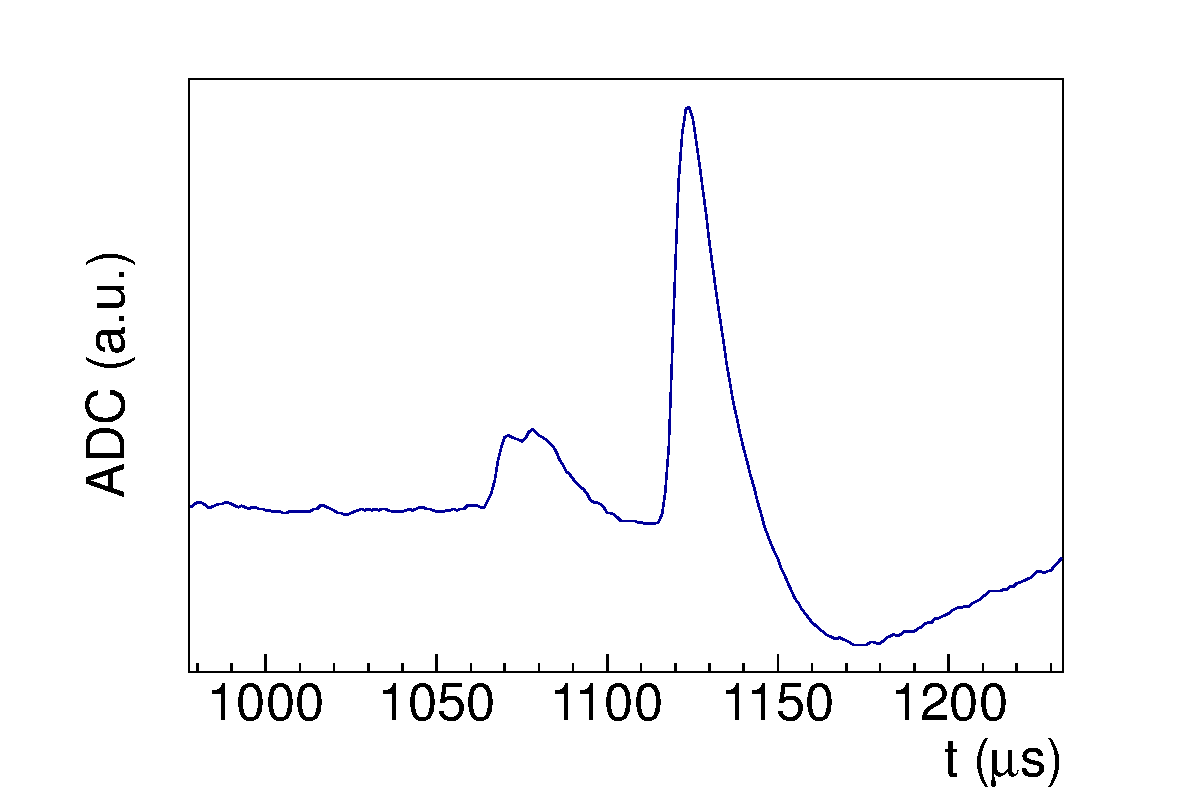
\includegraphics[width=\textwidth]{./plots/data_signal_finding_raw.pdf}
		\caption[Raw \(u\) wire waveform]{A raw \(u\) wire waveform showing two signals.}
		\label{fig:data_signal_finding_raw}
	\end{subfigure}\hfill%
	\begin{subfigure}[t]{0.48\textwidth}
		\centering
		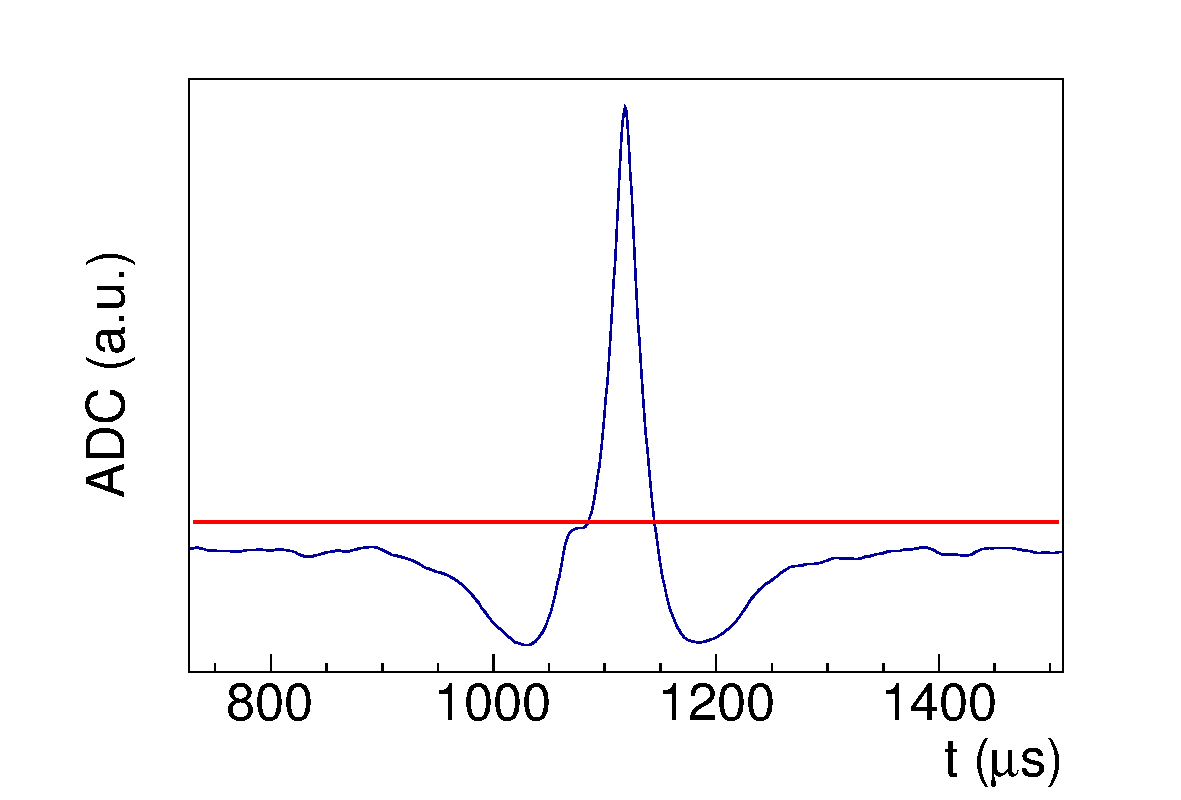
\includegraphics[width=\textwidth]{./plots/data_signal_finding_mf.pdf}
		\caption[Matched filter output]{The output of the matched filter with the threshold shown in red.}
		\label{fig:data_signal_finding_mf}
	\end{subfigure}
	\begin{subfigure}[t]{0.48\textwidth}
		\centering
		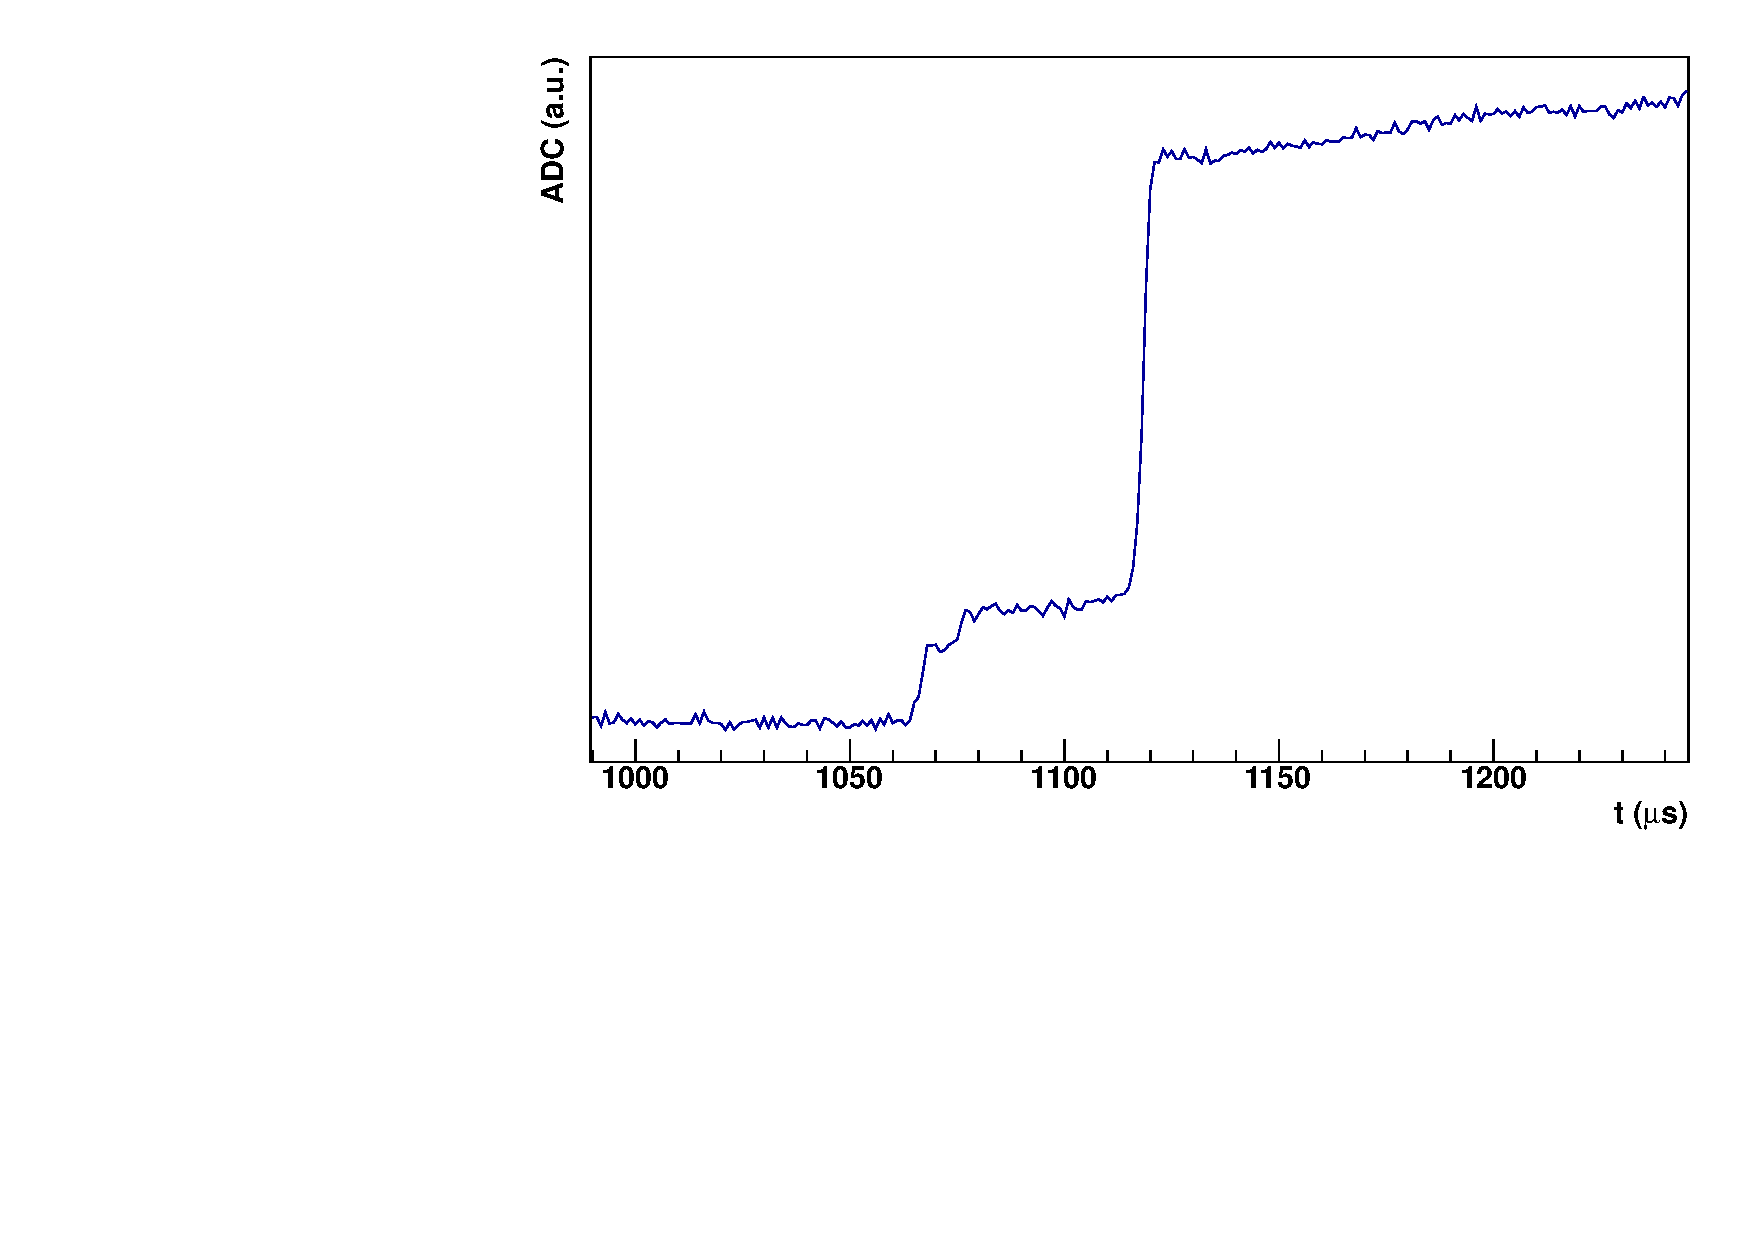
\includegraphics[width=\textwidth]{./plots/data_signal_finding_unshaped.pdf}
		\caption[Unshaped signals]{The `unshaped' signals.}
		\label{fig:data_signal_finding_unshaped}
	\end{subfigure}\hfill%
	\begin{subfigure}[t]{0.48\textwidth}
		\centering
		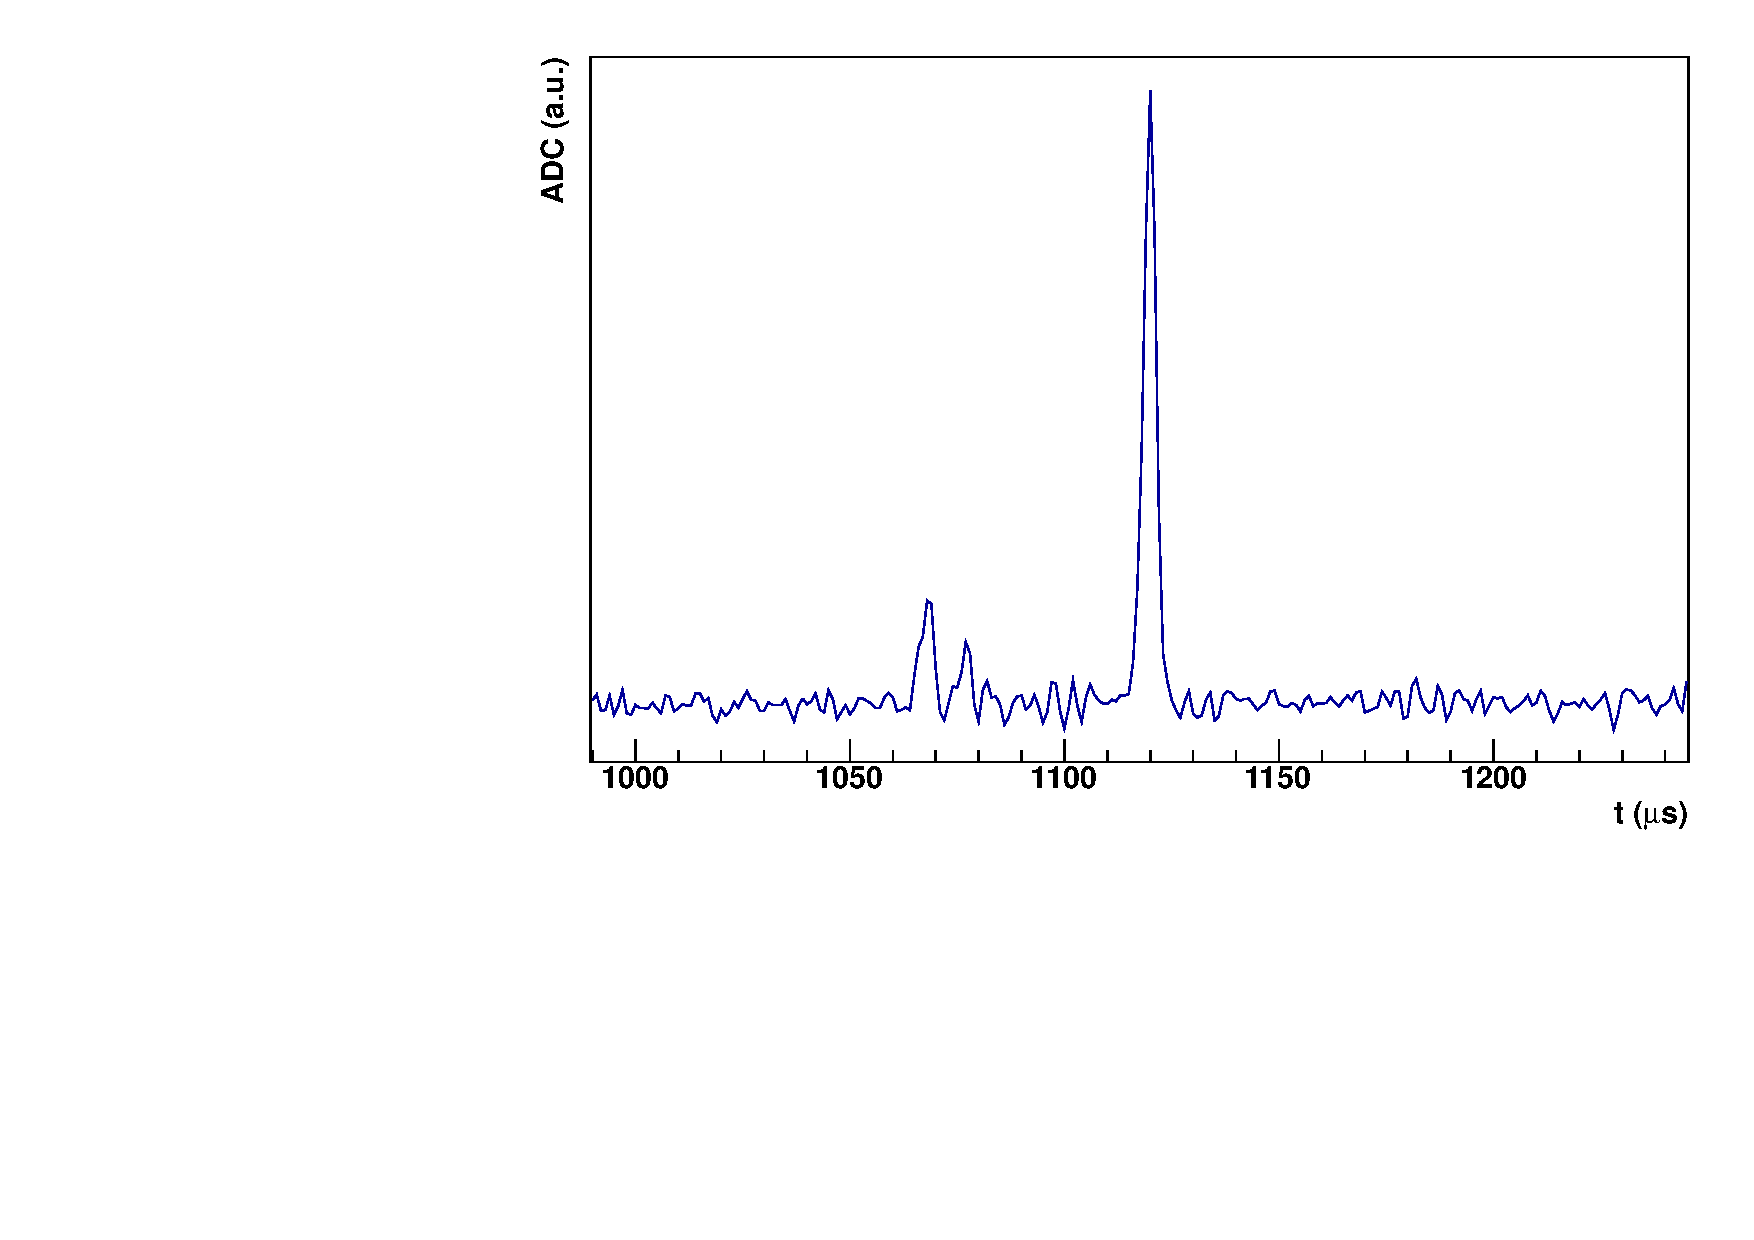
\includegraphics[width=\textwidth]{./plots/data_signal_finding_msf.pdf}
		\caption[Multiple signal finger output]{The output of a \SI{2}{\micro\s} triangular filter applied to the unshaped signals.}
		\label{fig:data_signal_finding_msf}
	\end{subfigure}
	\caption[The signal-finding process]{An example of finding signals on a \(u\) wire waveform.}
	\label{fig:data_signal_finding}
\end{figure}

The matched filter technique\cite{North:1963fk} convolves a time-reversed template signal with the waveform. Template signals are produced by passing a step function through the filters specified in \cref{tab:data_shaping_times}. This is done for individual channels for the \(u\) and \(v\) wires. For the APDs, the signals on the individual planes are summed and this technique is applied to these two sum signals. A threshold is determined by calculating the mean absolute deviation (MAD) of the waveform from its baseline. Parts of the waveform exceeding \((3\sqrt{\pi/2})\times\text{MAD}\) are excluded and the MAD is recalculated. A signal is found if the filter output exceeds 5 (4) times this final MAD for the wire (APD) signals. \Cref{fig:data_signal_finding_raw,fig:data_signal_finding_mf} show an example of this process.

While the matched filter is good at identifying that there was a signal on a wire, a refined analysis is needed to identify if multiple signals occurred in a short period of time. As \cref{fig:data_signal_finding_mf} shows, the matched filter only finds one signal when two are clearly visible. To find other signals, a \SI{256}{\micro\s} portion of the raw waveform is unshaped (by convolving the signal with the inverse transfer function of the shapers), then reshaped with a \SI{2}{\micro\s} triangular filter. Peaks in the output correspond to distinct signals. Finding multiple signals aids in discriminating against Compton-scattering \(\gamma\) ray backgrounds.

\subsection{Signal Parameter Extraction}
Once signals have been identified in a waveform, information about their energies and times are extracted by fitting template waveforms (determined by the shaping times in \cref{tab:data_shaping_times}) to the waveforms. This is done by minimizing the \(\chi^2\) statistic formed by comparing the baseline-subtracted waveform to the template waveform. Signals that fit to similar times are combined. Signals that fit to small amplitudes or have large errors on the fit amplitude are removed. Minimization is repeated until no more signals need to be combined or removed. This is done on the individual \(u\) and \(v\) wire channels, and on the two plane sum APD signals.

Signals that are collected on a \(u\) wire channel can induce signals in neighboring channels. These induction signals could be mistaken for collection signals. Induction signals are identified and removed by combining information from a number of metrics:
\begin{itemize}
\item The rise times and maximum-to-minimum times of the pulses in the waveforms are shorter for induction signals than collection signals.
\item The integrals of the unshaped waveforms are much larger for collection signals than induction signals.
\item Induction signals have a better \(\chi^2\) statistic when fit to a template induction signal than to a template collection signal.
\item Induction signals occur on channels that neighbor channels with very large collection signals (associated with events of \(\gtrsim\)~\SI{1}{\MeV}).
\end{itemize}

\subsection{Signal Clustering}
Once signals have been identified, signals of the same type may be bundled together:
\begin{itemize}
\item \(u\) wire signals: signals that are on neighboring channels and are within \SI{3.5}{\micro\s} of each other most likely came from the same energy deposition, and so are bundled together. This bundle is assigned the energy-weighted mean time and \(u\) position of the constituent signals.
\item \(v\) wire signals: induction effects from a single energy deposition may affect more than the nearest-neighbor channels. \(v\) wire signals are bundled together if \(|(t_{i} + (\SI{2.97}{\micro\s})\Delta v) - t_0|< \SI{4.5}{\micro\s}\), where \(t_0\) is the largest amplitude signal and \(\Delta v\) is the difference in channel number between the largest signal and signal \(i\). This is based on an empirical measurement that channels farther away from the event fit to earlier signal times. The resulting bundle is assigned the energy-weighted mean \(v\) position of the bundled signals and the time of the largest signal.
\item The sum APD plane signals are bundled together if they have times within \SI{6}{\micro\s} (based on the integration times for the shaping circuits). This bundle is assigned the energy-weighted mean time of the signals.
\end{itemize}

The \(z\) position of each \(u\) wire bundle is calculated using the time of the most recent scintillation bundle and the known drift velocity for ionization. If no scintillation bundle is found within the maximum physically possible drift time, the bundle is not assigned a \(z\) position. Later data quality cuts remove events that have more than one scintillation bundle within this time window, since the \(z\) position becomes ambiguous.

Finally, \(u\) signal bundles are paired with \(v\) signal bundles to form a ``cluster''. For each possible pairing, a likelihood is computed used 3 PDFs:
\begin{itemize}
\item After correcting for the known drift velocity between the anodes, the distribution of two paired \(u\) and \(v\) bundle times is a Gaussian centered around 0, with the standard deviation determined by the timing resolution of \SI{1}{\micro\s}.
\item The relationship between \(u\) and \(v\) signal magnitudes has been studied. Once the magnitudes of the bundles have been appropriately scaled, the distribution of their differences is again Gaussian, smeared by the energy resolution.
\item Not all \(u\) and \(v\) wire channels cross. If a pairing would cause the signal to be outside the hexagon containing the wires, the likelihood is penalized. The perpendicular distance to the edge of this hexagon is calculated. The penalty is the likelihood to be that distance away from the mean of a Gaussian distribution with standard deviation \SI{4.5}{\mm} (half the wire pitch).
\end{itemize}

The paired \(u\) and \(v\) bundles provide a 2D transverse position for the event. Since the wires do not cross at right angles, this position is translated to a \((x, y)\) position. The \(+y\) direction is vertically upward, the \(+x\) direction is away from the cryostat door, and \(+z\) is along the TPC axis and chosen to make the coordinate system right-handed. The position \((x, y, z) = (0, 0, 0)\) is defined to be the center of the detector, which is the center of the cathode.

\subsection{Topology}
\label{sec:data_topology}
An event may have zero, one, or many clusters. This proves a useful tool for discriminating beta decays from gamma ray backgrounds. The electron(s) from a beta decay deposit their energy in a small volume, creating mostly events with one cluster. A small fraction create bremsstrahlung photons that create multiple clusters. Meanwhile, gamma ray backgrounds tend to Compton scatter, producing events with multiple clusters. Some, however, do photoionize the xenon or Compton scatter in a small volume, producing only one cluster. When an electron-positron pair is created, if the \SI{511}{\keV} gamma rays from the positron annihilation escape the detector, this also only produces one cluster.

Two categories of event are created:
\begin{itemize}
\item Single Site (SS) events: events with only one cluster. Additionally, this cluster must have only occurred on two or fewer adjacent \(u\) wires. This selects most beta decay events and few gamma ray events.
\item Multiple Site (MS) events: events that are not single site. This selects most gamma ray events, with only a small number of beta decay events.
\end{itemize}

The clustering algorithm above is limited by the position resolution of the detector. For the \(u\) wires, the resolution is dominated by the \SI{9}{\mm} pitch. For the \(v\) wires, the magnitude of the induction signal on a channel is correlated with the signal's distance from that channel. Since induction signals occur on many neighboring channels, the \SI{9999}{\mm} resolution in \(v\) is better than for \(u\). The sampling frequency and shaping times determine the resolution in \(z\). With the multiple signal finder described about, the resolution is about \SI{9999}{\mm}.

\section{Corrections}
In order to have good energy resolution, events of the same energy should be reconstructed with the same energy, regardless of where in the detector they originated or on which channels the signals were collected. In order to achieve this, a number of corrections are applied to correct for both gain and positional variation. They are detailed below.

\subsection{Wire Gain Corrections}
\begin{figure}
	\begin{subfigure}[t]{0.48\textwidth}
		\centering
		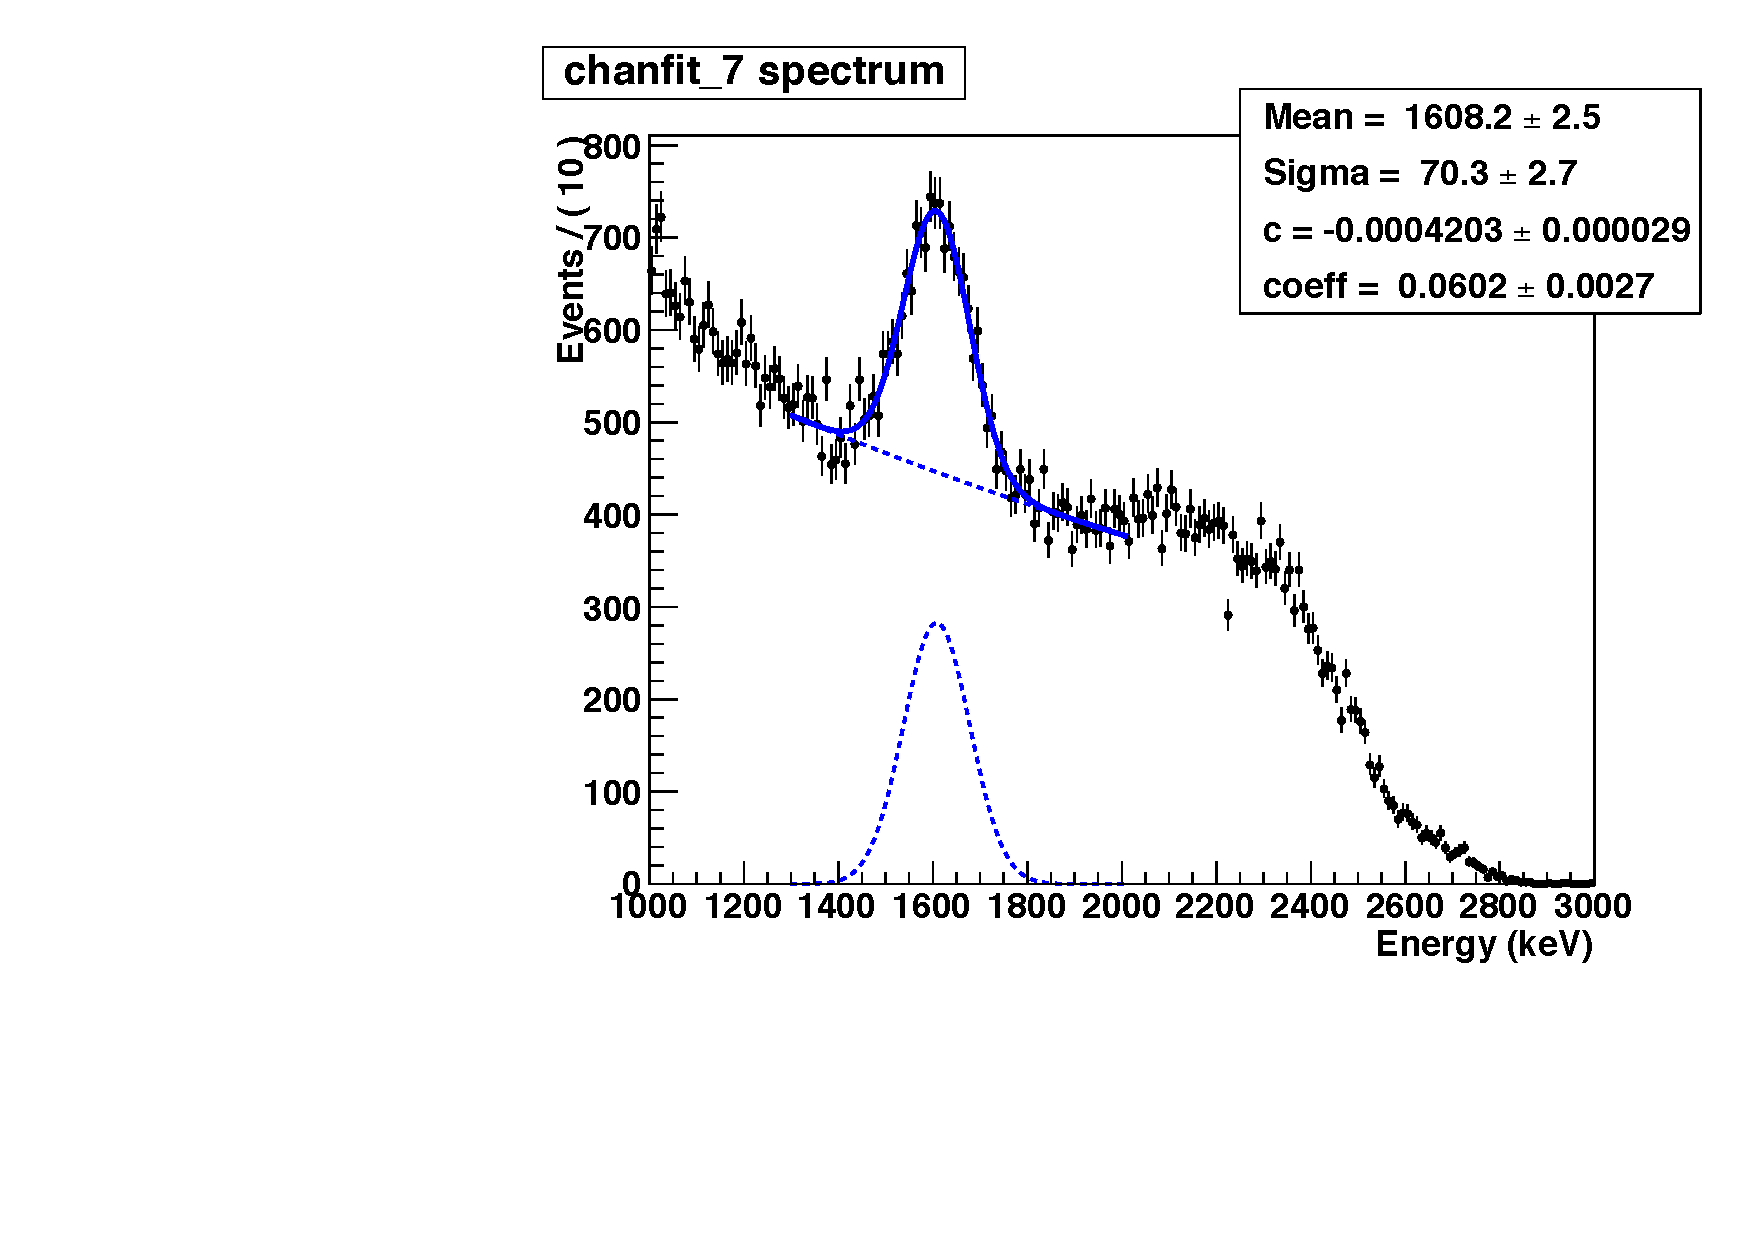
\includegraphics[width=\textwidth]{./plots/data_wiregain_pp07.pdf}
	\end{subfigure}\hfill%
	\begin{subfigure}[t]{0.48\textwidth}
		\centering
		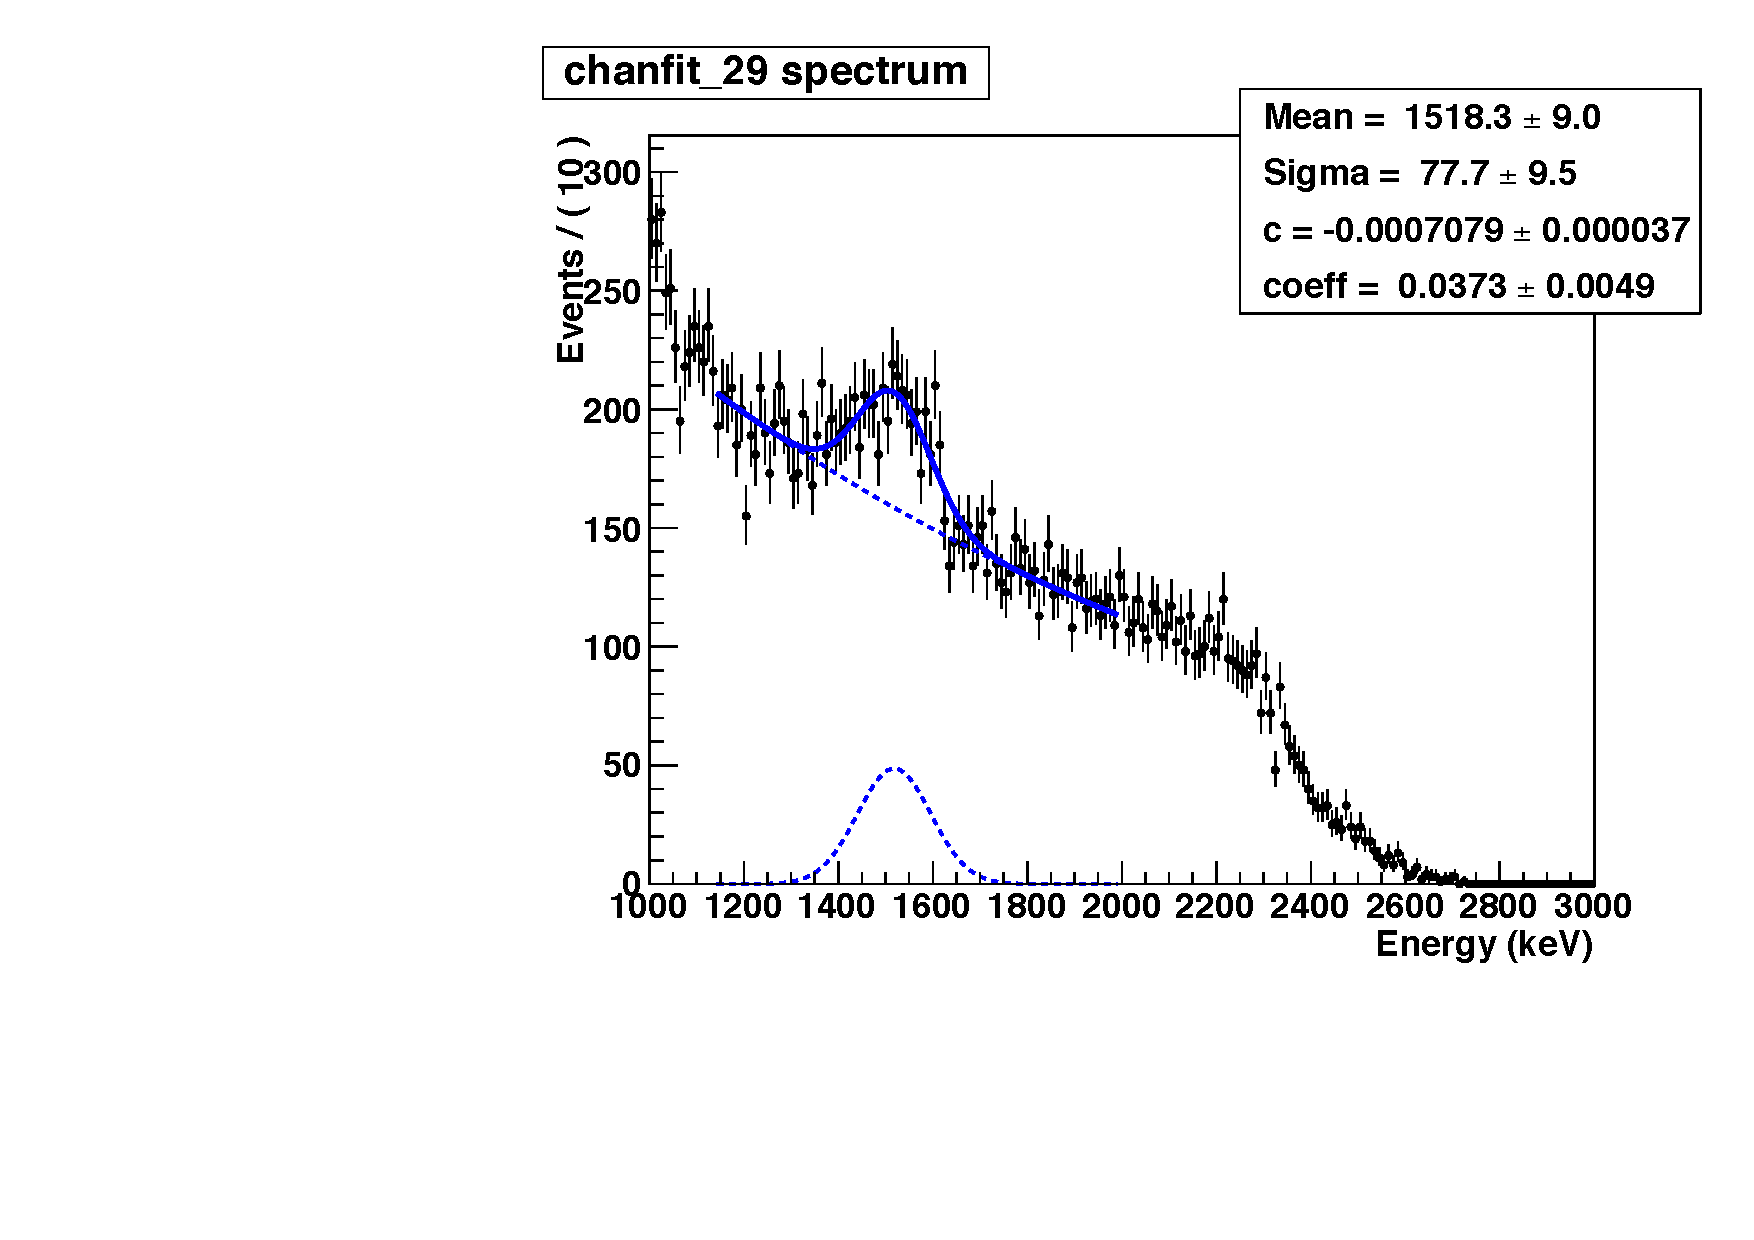
\includegraphics[width=\textwidth]{./plots/data_wiregain_pp29.pdf}
	\end{subfigure}
	\caption[The pair-production peak on individual \(u\) wire channels]{The \SI{1593}{\keV} pair-production peak shown on two different, uncorrected \(u\) wire channels. A Gaussian peak with an exponential background matches the observed spectrum well, and the mean obtained from the fit is then used to correct for channel-to-channel variations.}
	\label{fig:data_wiregain_pp}
\end{figure}

Minute differences in the components that read out each \(u\) wire channel can cause channel-to-channel variation in their responses. In order to address this, data from \thorium{228} calibration runs is used. The \SI{2615}{\keV} \(\gamma\) ray can produce an electron-positron pair with combined energy \SI{1593}{\keV}. Since the electron and positron deposit their energy in a small volume, this peak is clearly visible on individual wire channels. A scaling factor for each channel is determined by fitting these peaks and scaling so that they occur at the same value for each channel. \Cref{fig:data_wiregain_pp} shows examples for two channels.

Environmental conditions can also cause the response to shift over time. To address this, each channel has a capacitor that can inject a known amount of charge. These charge injections are done \about{} daily and used to measure the shaping time for the charge preamp (see \cref{sec:data_signal_readout}), but can also be used to measure the time variation of each individual channel. The time variation is tracked, and applied as a very small correction on top of the channel-to-channel correction.

\subsection{Shielding Grid Correction}
When ionization is created in a TPC, the positively charged ions move more slowly than the much less massive electrons. These positive ions can induce a signal on the collection wires opposite the collection signal. The measured signal will be reduced. For events far from the anode, the induction wire grid shields the collection wires from this effect. However, closer to the anode, the shielding grid is not perfect\cite{Bunemann:1949kx}, and so this effect must be corrected for.\todo{Fill in final details, whatever gets decided on.}

\subsection{Electron Lifetime Correction}
Ionization drifting in the TPC is attenuated by attachment to electronegative impurities. For uniformly distributed impurities, this results in an exponentially decreasing signal as a function of drift time, and the corresponding time constant is the ``electron lifetime''. This effect can be measured by measuring the attenuation of a known signal (as during a radioactive source calibration). This measurement is then used to correct unknown signals. \Cref{ch:electronlifetime} details the measurement of the electron lifetime and correction.

\subsection{Light Collection Correction}
While trim voltages are applied to the APDs to try to achieve a uniform response, there is still some variation in the gain from channel to channel. Additionally, there is geometric variation in the amount of scintillation light actually reaching the APDs due to shadowing from the wire planes, imperfect reflection off of the walls, and other effects. Using radioactive source calibration runs, the overall response from both of these factors can be mapped out and corrected for. \Cref{app:lightmap} details this correction.

\section{Energy Calibration}
\label{sec:data_calibration}
The calibration system described in \cref{sec:detector_calibration} is used to calibrate the energy scale of the detector. This is done separately for single site and multiple site events.
\subsection{Fit Model}
For gamma ray lines, a Gaussian distribution representing the full-absorption peak is combined with a complimentary error function representing Compton scatter events that escape the detector. Explicitly, the model is:
\begin{equation}
\frac{dN}{dE} = a \frac{1}{\sigma\sqrt{2\pi}}\exp\left(\frac{-(E-E_0)^2}{2\sigma^2}\right)+ (1-a)\text{erfc}\left(\frac{E-E_0}{\sqrt{2}\sigma}\right)
\label{eq:data_fitmodel}
\end{equation}
where the peak energy \(E_0\), width \(\sigma\), and peak fraction \(a\) are all allowed to float.

This model is fit to spectra collected in \isotope{137}{Cs} and  \thorium{228} calibrations, and a sum of two such models is fit to data from \isotope{60}{Co} calibrations, since it emits two gamma rays similar in energy. The energy spectra are fit using an unbinned maximum likelihood method. This fit is performed twice, first over a broad energy range to roughly identify the peak, then again in the range \((-3.0\sigma, +2.5\sigma)\) from the found peak to more precisely determine the mean energy, and to minimize bias introduced by the choice of fit window.

\begin{table}[htp]
\centering
\caption[Fit function biases]{The bias for fits using \cref{eq:data_fitmodel} obtained from Monte Carlo simulations of the sources. It is defined as \(E^\text{bias} = (E^\text{true} - E^\text{fit})\). It differs for single site (SS) and multiple site (MS) events.}
\label{tab:data_fit_biases}
\begin{tabular}{c c c c c}\toprule
	&	\multicolumn{4}{c}{\(E^\text{bias} = (E^\text{true} - E^\text{fit})\) (\si{\keV})}					\\\cmidrule{2-5}
	&	\isotope{137}{Cs} 	&	\multicolumn{2}{c}{\isotope{60}{Co}}			&	\isotope{228}{Th}	\\
	&	(at \SI{662}{\keV})	&	(at \SI{1173}{\keV})	&(at \SI{1333}{\keV})		&	(at \SI{2615}{\keV})	\\\midrule
SS 	& 	3.19				& 3.19				& 2.50				&	3.82 				\\
MS 	& 	8.13 				& 6.19 				& 6.35 				&	7.15				\\\bottomrule
\end{tabular}
\end{table}

This model exhibits a slight bias. That is, the mean energy found is different than the true value. This can be measured by applying the fit model to Monte Carlo simulations of the sources, where the true peak location is known. The biases are summarized in \cref{tab:data_fit_biases}. The bias varies as a function of energy resolution, and with the peak-to-Compton ratio, which is why it is not the same in all cases.

\subsection{Rotation Angle}
As described in \cref{sec:xe_combining_ion_and_scint}, the ionization and scintillation signals can be combined by projection onto a rotated axis in order to achieve good energy resolution. In order to determine the optimal angle, the energy spectra for calibration runs are constructed using a range of different angles using
\begin{equation}
E_R = E_{I}\cos\theta_R + E_{S}\sin\theta_R
\label{eq:data_E_rotated}
\end{equation}
where \(E_I\) and \(E_S\) are the ionization and scintillation signals after all corrections, but no calibrations, have been applied. The spectra are fit with the model in \cref{eq:data_fitmodel}, and the angle that optimizes the resolution \(\sigma/E_0\) is selected. \Cref{fig:data_finding_theta} shows an example of this process. Because \(E_I\) and \(E_S\) are uncalibrated, the value of \(\theta_R\) determined in this manner has no physical meaning.

\begin{figure}
	\begin{subfigure}[t]{0.48\textwidth}
		\centering
		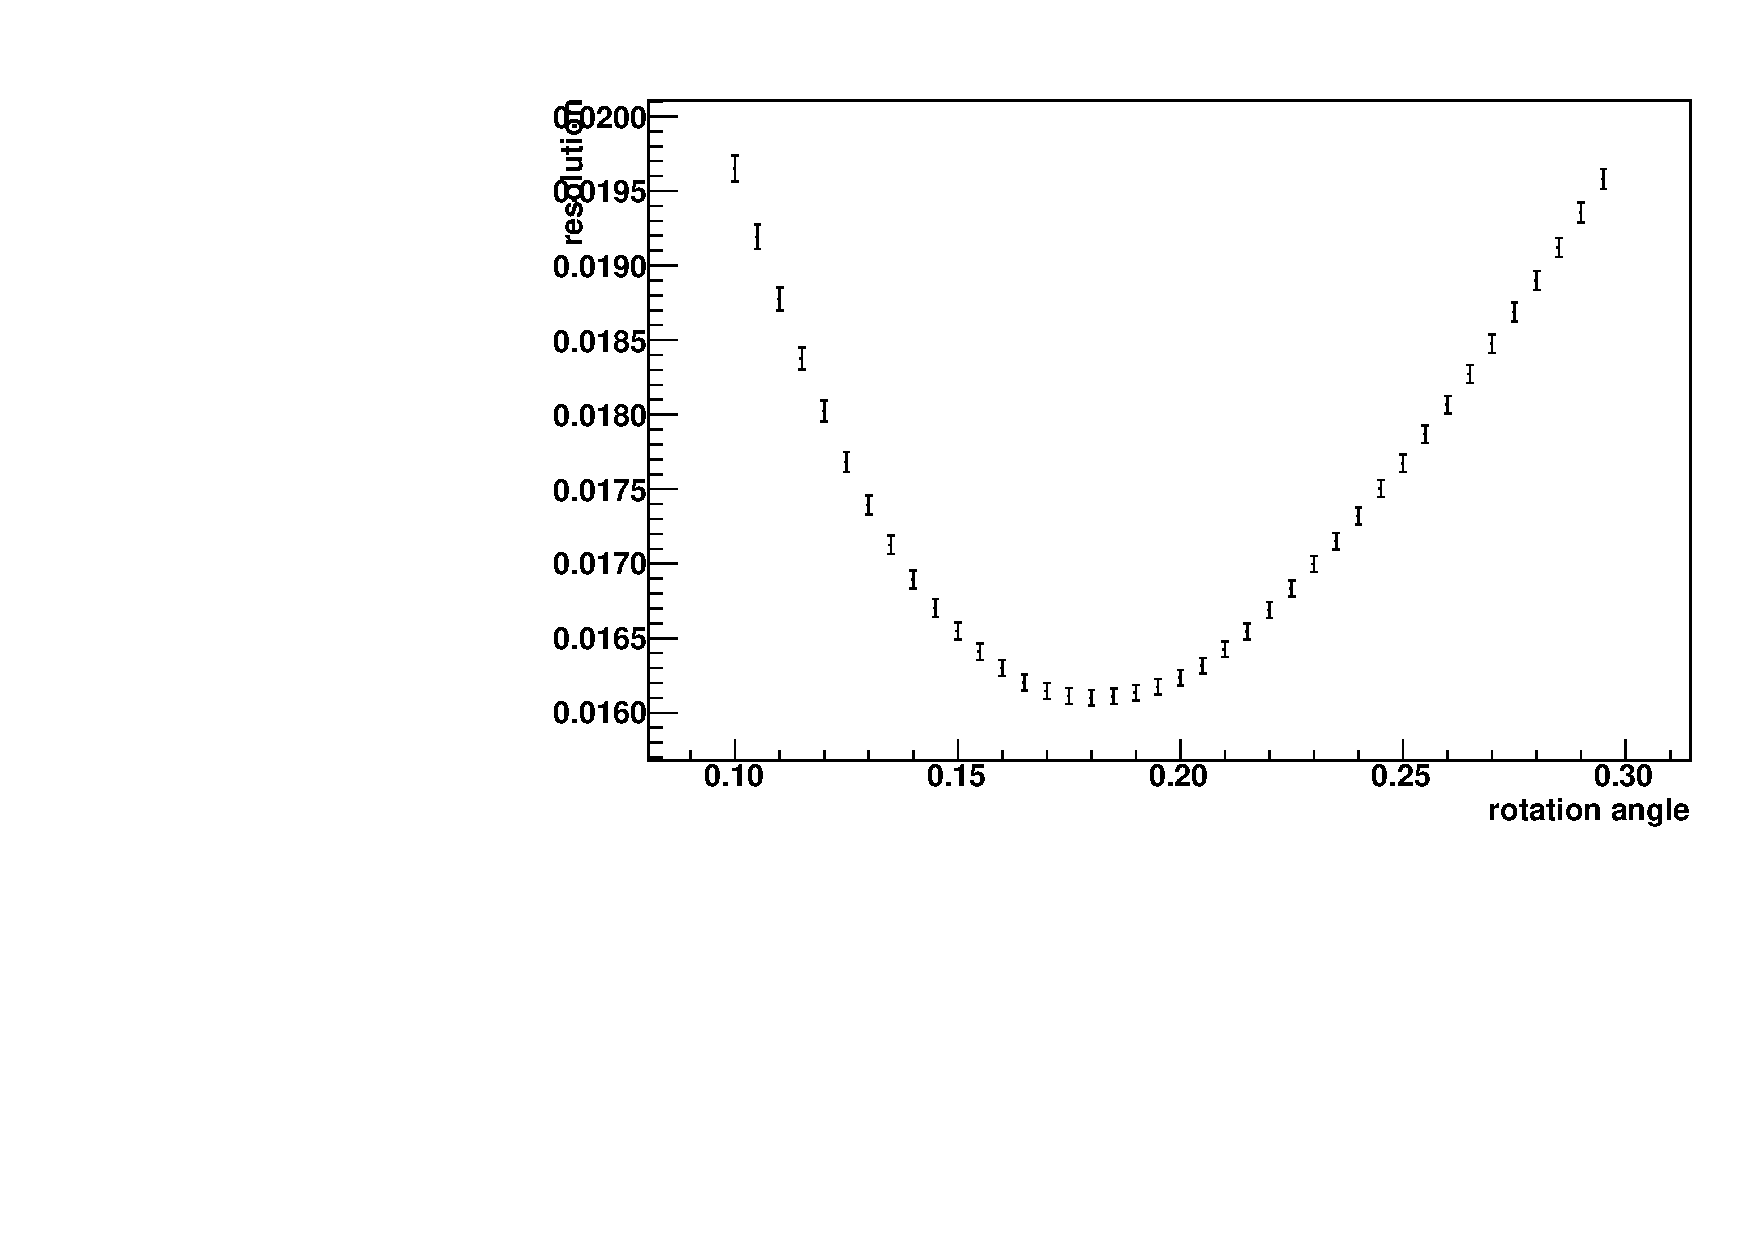
\includegraphics[width=\textwidth]{./plots/data_finding_theta_scan.pdf}
	\end{subfigure}\hfill%
	\begin{subfigure}[t]{0.48\textwidth}
		\centering
		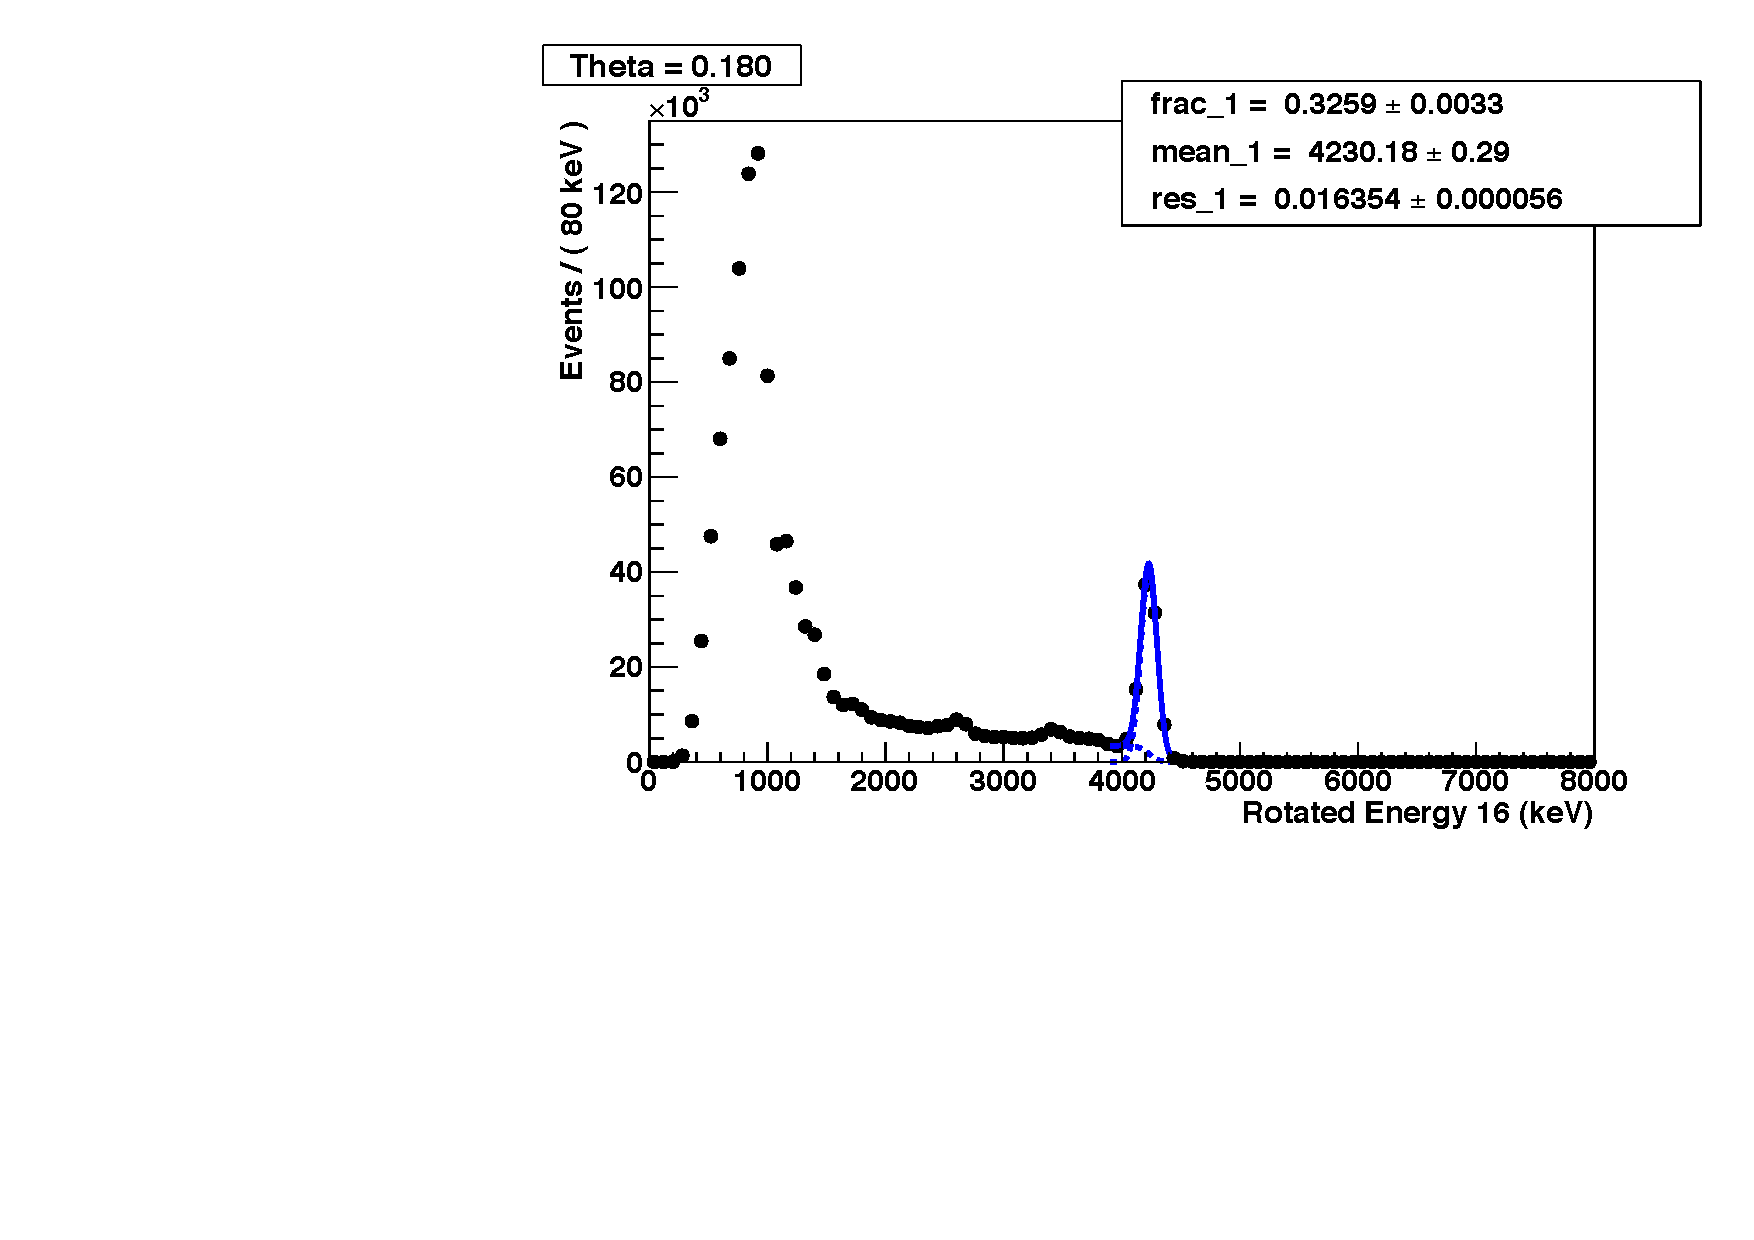
\includegraphics[width=\textwidth]{./plots/data_finding_theta_best.pdf}
	\end{subfigure}
	\caption[Finding the optimal rotation angle]{The rotation angle is scanned over a range of values (left) in order to find the angle that optimizes rotation. In this case, the optimal angle was \(\theta = 0.18\). On the right, the fit of the model in \cref{eq:data_fitmodel} to thorium calibration data with the optimal rotation applied (according to \cref{eq:data_E_rotated}).}
	\label{fig:data_finding_theta}
\end{figure}

\subsection{Thorium Peak}
Thorium source calibrations are taken every 1--2~days. On a week-by-week basis, the optimal rotation angle for the \SI{2615}{\keV} full absorption peak is determined from these calibrations. This angle is used for all data during that week. \SI{2615}{\keV} is close to the \SI{2458}{\keV} Q value for \xenon{136}, and so optimizing the resolution for the thorium peak should also give good resolution near the \zeronu{} peak.


\subsection{Overall Energy Scale}
While thorium source calibrations are taken frequently, the cobalt and cesium sources are generally reserved for dedicated campaigns. Throughout these campaigns, it has been observed that the ratio between the peak energies remain relatively stable, even though their values show some drift. This is shown in \cref{fig:data_energy_ratios_time}. Therefore, the three ratios \(E_\text{Cs}/E_\text{Th}\) and \(E_{\text{Co},i}/E_\text{Th}\) are used as the basis for the calibration. The process for calibration is then:
\begin{enumerate}
\item On a week-by-week basis, use thorium calibration data to determine the optimal rotation angle \(\theta(t)\) and to fit the thorium peak \(E^\text{fit}_\text{Th}(t)\) in the spectrum obtained using \cref{eq:data_E_rotated} and that rotation angle. If no thorium data is available for a given week, data from the adjacent weeks are combined and used to estimate the angle and peak for that week.
\item For each multiple isotope calibration campaign, compute the ratios \(E^\text{fit}_\text{Cs}/E^\text{fit}_\text{Th}\) and \(E^\text{fit}_{\text{Co},i}/E^\text{fit}_\text{Th}\)
\item Using the mean values from these campaigns and the true ratios, fit a polynomial function \(f\) such that \(f([E^\text{fit}/E^\text{fit}_\text{Th}]|_\text{data}) = [E^\text{fit}/E^\text{fit}_\text{Th}]|_\text{simulation}\). The ratios used for this fit are shown in \cref{tab:data_calib_ratios}.
\end{enumerate}

\begin{table}[htp]
\centering
\caption[Calibration peak ratios]{The mean ratios of the fitted Cs and Co peaks to the Th peaks taken from calibration campaigns. The error on data is the RMS of the ratios from the campaigns.}
\label{tab:data_calib_ratios}
\begin{tabular}{r r c c c c c}\toprule
				&				&	\multicolumn{2}{c}{Single Site}	&	\multicolumn{2}{c}{Multiple Site}		\\\cmidrule(lr){3-4}\cmidrule(lr){5-6}
isotope			&	E (\si{\keV})	&	data					&	simulation		&	data					&	simulation	\\\midrule
\isotope{137}{Cs}	&	662 			& \num{0.2513\pm0.0007}	& 0.2523 			& \num{0.2496\pm0.0009}	&	0.2507 	\\
\isotope{60}{Co}	& 	1173			& \num{0.4488\pm0.0007}	& 0.4480 			& \num{0.4488\pm0.0006}	&	0.4474 	\\
\isotope{60}{Co}	& 	1333			& \num{0.5109\pm0.0008}	& 0.5095 			& \num{0.5100\pm0.0004}	&	0.5087 	\\\bottomrule
\end{tabular}
\end{table}


The calibrated energy of an event, then, with rotated energy \(E_R(\theta(t))\) is (taking into account the fit function bias)
\begin{equation}
E = \left(E^\text{true}_\text{Th} - E^\text{bias}_\text{Th}\right) f\left(\frac{E_R(\theta(t))}{E^\text{fit}_\text{Th}(t)}\right)
\label{eq:data_E_calibration}
\end{equation}
where
\begin{equation}
f(x) = \begin{dcases*}
	5.17\times10^{-3} + 0.9797 \cdot x + 1.516\times10^{-2} \cdot x^2	&	(single-site events)	\\
	5.37\times10^{-3} + 0.9784 \cdot x + 1.635\times10^{-2} \cdot x^2	&	(multi-site events)
	\end{dcases*}
\end{equation}
The residuals from the calibration campaigns are shown in \cref{fig:data_calibration_residuals}. This ratio-based method allows for some correction of the time variation without requiring additional time to be spent calibrating.
\begin{figure}[htp]
	\centering
	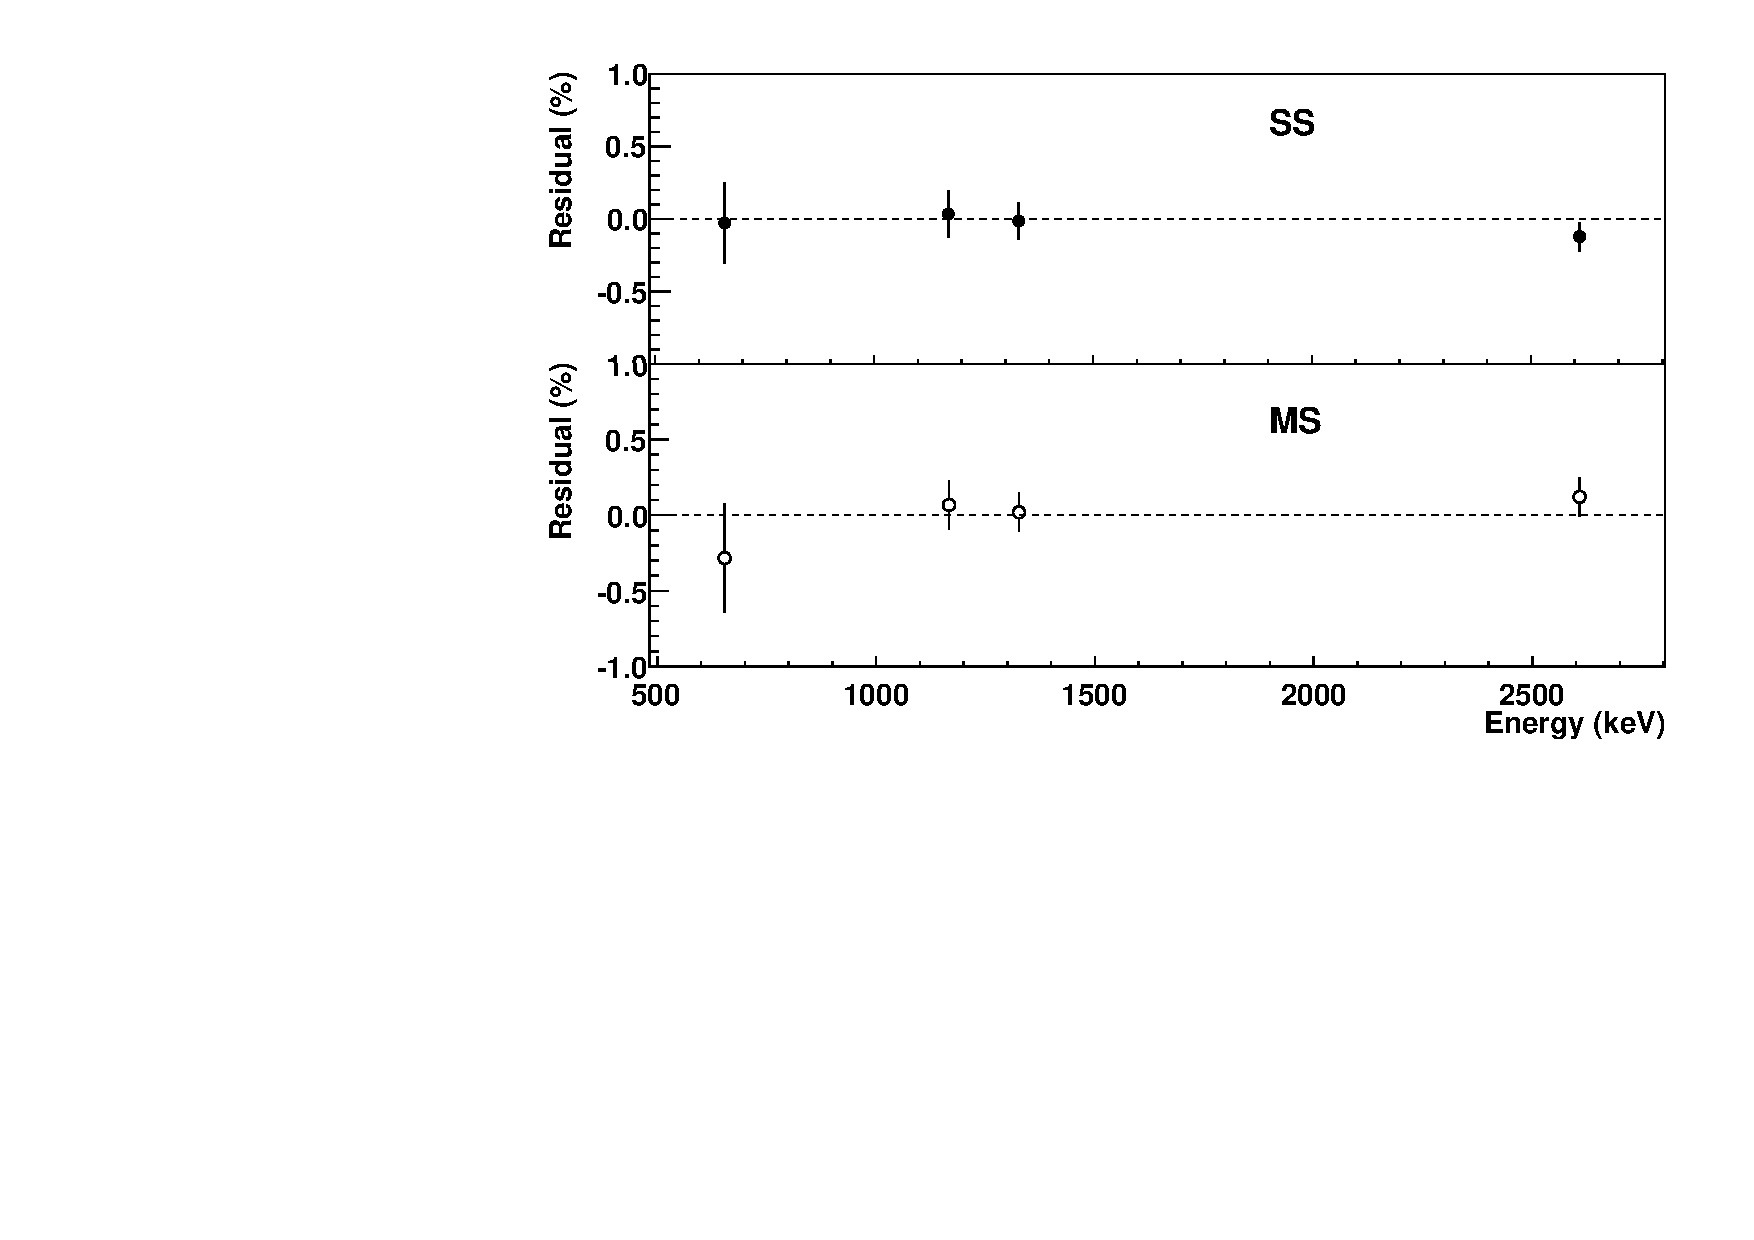
\includegraphics[width=0.8\textwidth]{./plots/data_calibration_residuals.pdf}
	\caption[Residuals of energy calibration]{The residuals \((E^\text{fit} - E^\text{true})/E^\text{true}\) for the calibration source peaks after the calibration is applied. The top shows them for the single site calibration, while the bottom shows them for the multiple site calibration. The points are the mean of all source calibration campaigns, while the error bars represent the RMS.}
	\label{fig:data_calibration_residuals}
\end{figure}

\section{Data Quality Cuts}
Once the data has been processed, a number of data quality cuts are applied before it can be used in analyses. These cuts help ensure that the detector response and behavior are consistent throughout the data set. Summarizing them:
\begin{itemize}
\item The DAQ must be operating normally. All voltages must be nominal, and the trigger must be the standard one. Channels must not have an unusual baseline or RMS (indicating high noise).
\item The number of forced \SI{0.1}{\Hz} triggers must be consistent with the DAQ recorded start and end time for the data run.
\item The rate at which the DAQ records triggers must not be unusually high or low. Individual channels must not be creating abnormally many or few triggers.
\item The active muon veto must be operational.
\item The electron lifetime in the TPC must be good and not changing rapidly. The considerations behind this cut are explained in \cref{sec:el_practical_considerations}.
\item The rate of events that cannot be reconstructed (as in \cref{sec:data_reconstruction}) must be small.
\item The rate of events with energies greater than \SI{300}{\keV}, \SI{1000}{\keV}, and \SI{2000}{\keV} should not vary significantly from previously observed rates.
\item The run must be long enough (\SI{1800}{\s}) that the above criteria can be properly evaluated.
\end{itemize}

\end{document}
